
%% bare_conf.tex
%% V1.4b
%% 2015/08/26
%% by Michael Shell
%% See:
%% http://www.michaelshell.org/
%% for current contact information.
%%
%% This is a skeleton file demonstrating the use of IEEEtran.cls
%% (requires IEEEtran.cls version 1.8b or later) with an IEEE
%% conference paper.
%%
%% Support sites:
%% http://www.michaelshell.org/tex/ieeetran/
%% http://www.ctan.org/pkg/ieeetran
%% and
%% http://www.ieee.org/

%%*************************************************************************
%% Legal Notice:
%% This code is offered as-is without any warranty either expressed or
%% implied; without even the implied warranty of MERCHANTABILITY or
%% FITNESS FOR A PARTICULAR PURPOSE! 
%% User assumes all risk.
%% In no event shall the IEEE or any contributor to this code be liable for
%% any damages or losses, including, but not limited to, incidental,
%% consequential, or any other damages, resulting from the use or misuse
%% of any information contained here.
%%
%% All comments are the opinions of their respective authors and are not
%% necessarily endorsed by the IEEE.
%%
%% This work is distributed under the LaTeX Project Public License (LPPL)
%% ( http://www.latex-project.org/ ) version 1.3, and may be freely used,
%% distributed and modified. A copy of the LPPL, version 1.3, is included
%% in the base LaTeX documentation of all distributions of LaTeX released
%% 2003/12/01 or later.
%% Retain all contribution notices and credits.
%% ** Modified files should be clearly indicated as such, including  **
%% ** renaming them and changing author support contact information. **
%%*************************************************************************


% *** Authors should verify (and, if needed, correct) their LaTeX system  ***
% *** with the testflow diagnostic prior to trusting their LaTeX platform ***
% *** with production work. The IEEE's font choices and paper sizes can   ***
% *** trigger bugs that do not appear when using other class files.       ***                          ***
% The testflow support page is at:
% http://www.michaelshell.org/tex/testflow/



\documentclass[conference]{IEEEtran}
% Some Computer Society conferences also require the compsoc mode option,
% but others use the standard conference format.
%
% If IEEEtran.cls has not been installed into the LaTeX system files,
% manually specify the path to it like:
% \documentclass[conference]{../sty/IEEEtran}





% Some very useful LaTeX packages include:
% (uncomment the ones you want to load)


% *** MISC UTILITY PACKAGES ***
%
%\usepackage{ifpdf}
% Heiko Oberdiek's ifpdf.sty is very useful if you need conditional
% compilation based on whether the output is pdf or dvi.
% usage:
% \ifpdf
%   % pdf code
% \else
%   % dvi code
% \fi
% The latest version of ifpdf.sty can be obtained from:
% http://www.ctan.org/pkg/ifpdf
% Also, note that IEEEtran.cls V1.7 and later provides a builtin
% \ifCLASSINFOpdf conditional that works the same way.
% When switching from latex to pdflatex and vice-versa, the compiler may
% have to be run twice to clear warning/error messages.






% *** CITATION PACKAGES ***
%
\usepackage{cite}
% cite.sty was written by Donald Arseneau
% V1.6 and later of IEEEtran pre-defines the format of the cite.sty package
% \cite{} output to follow that of the IEEE. Loading the cite package will
% result in citation numbers being automatically sorted and properly
% "compressed/ranged". e.g., [1], \cite{rubinsztejn_framework_2005}, \cite{gamma_design_1995}, \cite{holder_system_1999}, \cite{pratikakis_transparent_2004}, \cite{_fusion_????} without using
% cite.sty will become [1], \cite{gamma_design_1995}, \cite{pratikakis_transparent_2004}--\cite{holder_system_1999}, \cite{rubinsztejn_framework_2005} using cite.sty. cite.sty's
% \cite will automatically add leading space, if needed. Use cite.sty's
% noadjust option (cite.sty V3.8 and later) if you want to turn this off
% such as if a citation ever needs to be enclosed in parenthesis.
% cite.sty is already installed on most LaTeX systems. Be sure and use
% version 5.0 (2009-03-20) and later if using hyperref.sty.
% The latest version can be obtained at:
% http://www.ctan.org/pkg/cite
% The documentation is contained in the cite.sty file itself.






% *** GRAPHICS RELATED PACKAGES ***
%
\ifCLASSINFOpdf
  \usepackage[pdftex]{graphicx}
  % declare the path(s) where your graphic files are
  % \graphicspath{{../pdf/}{../jpeg/}}
  % and their extensions so you won't have to specify these with
  % every instance of \includegraphics
  \DeclareGraphicsExtensions{.pdf,.jpeg,.png}
\else
  % or other class option (dvipsone, dvipdf, if not using dvips). graphicx
  % will default to the driver specified in the system graphics.cfg if no
  % driver is specified.
  \usepackage[dvips]{graphicx}
  % declare the path(s) where your graphic files are
  % \graphicspath{{../eps/}}
  % and their extensions so you won't have to specify these with
  % every instance of \includegraphics
  \DeclareGraphicsExtensions{.eps}
\fi
% graphicx was written by David Carlisle and Sebastian Rahtz. It is
% required if you want graphics, photos, etc. graphicx.sty is already
% installed on most LaTeX systems. The latest version and documentation
% can be obtained at: 
% http://www.ctan.org/pkg/graphicx
% Another good source of documentation is "Using Imported Graphics in
% LaTeX2e" by Keith Reckdahl which can be found at:
% http://www.ctan.org/pkg/epslatex
%
% latex, and pdflatex in dvi mode, support graphics in encapsulated
% postscript (.eps) format. pdflatex in pdf mode supports graphics
% in .pdf, .jpeg, .png and .mps (metapost) formats. Users should ensure
% that all non-photo figures use a vector format (.eps, .pdf, .mps) and
% not a bitmapped formats (.jpeg, .png). The IEEE frowns on bitmapped formats
% which can result in "jaggedy"/blurry rendering of lines and letters as
% well as large increases in file sizes.
%
% You can find documentation about the pdfTeX application at:
% http://www.tug.org/applications/pdftex





% *** MATH PACKAGES ***
%
\usepackage{amsmath}
% A popular package from the American Mathematical Society that provides
% many useful and powerful commands for dealing with mathematics.
%
% Note that the amsmath package sets \interdisplaylinepenalty to 10000
% thus preventing page breaks from occurring within multiline equations. Use:
%\interdisplaylinepenalty=2500
% after loading amsmath to restore such page breaks as IEEEtran.cls normally
% does. amsmath.sty is already installed on most LaTeX systems. The latest
% version and documentation can be obtained at:
% http://www.ctan.org/pkg/amsmath





% *** SPECIALIZED LIST PACKAGES ***
%
\usepackage{algorithmic}
% algorithmic.sty was written by Peter Williams and Rogerio Brito.
% This package provides an algorithmic environment fo describing algorithms.
% You can use the algorithmic environment in-text or within a figure
% environment to provide for a floating algorithm. Do NOT use the algorithm
% floating environment provided by algorithm.sty (by the same authors) or
% algorithm2e.sty (by Christophe Fiorio) as the IEEE does not use dedicated
% algorithm float types and packages that provide these will not provide
% correct IEEE style captions. The latest version and documentation of
% algorithmic.sty can be obtained at:
% http://www.ctan.org/pkg/algorithms
% Also of interest may be the (relatively newer and more customizable)
% algorithmicx.sty package by Szasz Janos:
% http://www.ctan.org/pkg/algorithmicx




% *** ALIGNMENT PACKAGES ***
%
\usepackage{array}
% Frank Mittelbach's and David Carlisle's array.sty patches and improves
% the standard LaTeX2e array and tabular environments to provide better
% appearance and additional user controls. As the default LaTeX2e table
% generation code is lacking to the point of almost being broken with
% respect to the quality of the end results, all users are strongly
% advised to use an enhanced (at the very least that provided by array.sty)
% set of table tools. array.sty is already installed on most systems. The
% latest version and documentation can be obtained at:
% http://www.ctan.org/pkg/array


% IEEEtran contains the IEEEeqnarray family of commands that can be used to
% generate multiline equations as well as matrices, tables, etc., of high
% quality.




% *** SUBFIGURE PACKAGES ***
\ifCLASSOPTIONcompsoc
  \usepackage[caption=false,font=normalsize,labelfont=sf,textfont=sf]{subfig}
\else
  \usepackage[caption=false,font=footnotesize]{subfig}
\fi
% subfig.sty, written by Steven Douglas Cochran, is the modern replacement
% for subfigure.sty, the latter of which is no longer maintained and is
% incompatible with some LaTeX packages including fixltx2e. However,
% subfig.sty requires and automatically loads Axel Sommerfeldt's caption.sty
% which will override IEEEtran.cls' handling of captions and this will result
% in non-IEEE style figure/table captions. To prevent this problem, be sure
% and invoke subfig.sty's "caption=false" package option (available since
% subfig.sty version 1.3, 2005/06/28) as this is will preserve IEEEtran.cls
% handling of captions.
% Note that the Computer Society format requires a larger sans serif font
% than the serif footnote size font used in traditional IEEE formatting
% and thus the need to invoke different subfig.sty package options depending
% on whether compsoc mode has been enabled.
%
% The latest version and documentation of subfig.sty can be obtained at:
% http://www.ctan.org/pkg/subfig




% *** FLOAT PACKAGES ***
%
\usepackage{fixltx2e}
% fixltx2e, the successor to the earlier fix2col.sty, was written by
% Frank Mittelbach and David Carlisle. This package corrects a few problems
% in the LaTeX2e kernel, the most notable of which is that in current
% LaTeX2e releases, the ordering of single and double column floats is not
% guaranteed to be preserved. Thus, an unpatched LaTeX2e can allow a
% single column figure to be placed prior to an earlier double column
% figure.
% Be aware that LaTeX2e kernels dated 2015 and later have fixltx2e.sty's
% corrections already built into the system in which case a warning will
% be issued if an attempt is made to load fixltx2e.sty as it is no longer
% needed.
% The latest version and documentation can be found at:
% http://www.ctan.org/pkg/fixltx2e


\usepackage{stfloats}
% stfloats.sty was written by Sigitas Tolusis. This package gives LaTeX2e
% the ability to do double column floats at the bottom of the page as well
% as the top. (e.g., "\begin{figure*}[!b]" is not normally possible in
% LaTeX2e). It also provides a command:
%\fnbelowfloat
% to enable the placement of footnotes below bottom floats (the standard
% LaTeX2e kernel puts them above bottom floats). This is an invasive package
% which rewrites many portions of the LaTeX2e float routines. It may not work
% with other packages that modify the LaTeX2e float routines. The latest
% version and documentation can be obtained at:
% http://www.ctan.org/pkg/stfloats
% Do not use the stfloats baselinefloat ability as the IEEE does not allow
% \baselineskip to stretch. Authors submitting work to the IEEE should note
% that the IEEE rarely uses double column equations and that authors should try
% to avoid such use. Do not be tempted to use the cuted.sty or midfloat.sty
% packages (also by Sigitas Tolusis) as the IEEE does not format its papers in
% such ways.
% Do not attempt to use stfloats with fixltx2e as they are incompatible.
% Instead, use Morten Hogholm'a dblfloatfix which combines the features
% of both fixltx2e and stfloats:
%
% \usepackage{dblfloatfix}
% The latest version can be found at:
% http://www.ctan.org/pkg/dblfloatfix




% *** PDF, URL AND HYPERLINK PACKAGES ***
%
\usepackage{url}
% url.sty was written by Donald Arseneau. It provides better support for
% handling and breaking URLs. url.sty is already installed on most LaTeX
% systems. The latest version and documentation can be obtained at:
% http://www.ctan.org/pkg/url
% Basically, \url{my_url_here}.



\usepackage{hyperref}

\usepackage{minted}
\usepackage{tcolorbox}
\usepackage{etoolbox}
\BeforeBeginEnvironment{minted}{\begin{tcolorbox}}%
\AfterEndEnvironment{minted}{\end{tcolorbox}}%
\AtBeginEnvironment{minted}{\fontsize{8}{8}}




% *** Do not adjust lengths that control margins, column widths, etc. ***
% *** Do not use packages that alter fonts (such as pslatex).         ***
% There should be no need to do such things with IEEEtran.cls V1.6 and later.
% (Unless specifically asked to do so by the journal or conference you plan
% to submit to, of course. )


% correct bad hyphenation here
\hyphenation{op-tical net-works semi-conduc-tor}


\begin{document}
%
% paper title
% Titles are generally capitalized except for words such as a, an, and, as,
% at, but, by, for, in, nor, of, on, or, the, to and up, which are usually
% not capitalized unless they are the first or last word of the title.
% Linebreaks \\ can be used within to get better formatting as desired.
% Do not put math or special symbols in the title.
\title{Design and Implementation Mobile Data Collection\\Using Mobile Proxy}


% author names and affiliations
% use a multiple column layout for up to three different
% affiliations
\author{
\IEEEauthorblockN{Aris Prawisudatama}
\IEEEauthorblockA{School of Electrical Engineering and Informatics\\
Institut Teknologi Bandung\\
Bandung, Indonesia\\
Email: soedomoto@gmail.com}
\and
\IEEEauthorblockN{I Gusti Bagus Baskara Nugraha}
\IEEEauthorblockA{School of Electrical Engineering and Informatics\\
Institut Teknologi Bandung\\
Bandung, Indonesia\\
Email: baskara@stei.itb.ac.id}
}

% conference papers do not typically use \thanks and this command
% is locked out in conference mode. If really needed, such as for
% the acknowledgment of grants, issue a \IEEEoverridecommandlockouts
% after \documentclass

% for over three affiliations, or if they all won't fit within the width
% of the page, use this alternative format:
% 
%\author{\IEEEauthorblockN{Michael Shell\IEEEauthorrefmark{1},
%Homer Simpson\IEEEauthorrefmark{2},
%James Kirk\IEEEauthorrefmark{3}, 
%Montgomery Scott\IEEEauthorrefmark{3} and
%Eldon Tyrell\IEEEauthorrefmark{4}}
%\IEEEauthorblockA{\IEEEauthorrefmark{1}School of Electrical and Computer Engineering\\
%Georgia Institute of Technology,
%Atlanta, Georgia 30332--0250\\ Email: see http://www.michaelshell.org/contact.html}
%\IEEEauthorblockA{\IEEEauthorrefmark{2}Twentieth Century Fox, Springfield, USA\\
%Email: homer@thesimpsons.com}
%\IEEEauthorblockA{\IEEEauthorrefmark{3}Starfleet Academy, San Francisco, California 96678-2391\\
%Telephone: (800) 555--1212, Fax: (888) 555--1212}
%\IEEEauthorblockA{\IEEEauthorrefmark{4}Tyrell Inc., 123 Replicant Street, Los Angeles, California 90210--4321}}




% use for special paper notices
%\IEEEspecialpapernotice{(Invited Paper)}




% make the title area
\maketitle

% As a general rule, do not put math, special symbols or citations
% in the abstract
\begin{abstract}
Data collection using mobile device is something that is quite common recently. However, most of those applications are using static validation rules. The use of mobile proxy to duplicate rule and data is believed could improve the flexibility and implementation of the validation rule. Rule could be easily designed in modular basis, installed, updated, as well as deleted from application using OSGi framework. This paper is aimed to research about the design and implementation of mobile proxy that could be used to implement dynamic validation rule on SOA-based mobile device.
\end{abstract}

% no keywords




% For peer review papers, you can put extra information on the cover
% page as needed:
% \ifCLASSOPTIONpeerreview
% \begin{center} \bfseries EDICS Category: 3-BBND \end{center}
% \fi
%
% For peerreview papers, this IEEEtran command inserts a page break and
% creates the second title. It will be ignored for other modes.
\IEEEpeerreviewmaketitle




\section{Introduction}
Data collection is one of the main tasks of statistical institution in the world, including BPS-Statistics Indonesia. Data collection process is conducted using various media, ranging from conventional method, such as paper questionnaire to the modern method using mobile device. Until now, most of data collection conducted by BPS-Statistics Indonesia are still using paper questionnaire. However, BPS is now starting using mobile device for collecting data.

In data collection, the most important thing to be considered is the data quality. Data quality is measured using consistency and validation parameter. Data collection using paper questionnaire still rely on human’s carefulness and thoroughness in implementing the rule. Using mobile device has a benefit related to consistency and validation. Thus, generally, using mobile device could increase data quality.

The scenario that is commonly used in the implementation of mobile device application is to wrap it in a package including GUI and workflow. This scenario has a weakness, that workflows are used are static and cannot be added, removed, or updated, except by updating the whole application.

Another scenario which is also commonly used is by adopting a Service-Oriented approach. Service oriented approach basically separated into two components: the service provider (server) and a service consumer (client). In service-based approach, the workflow will be executed on the server, while the client access the workflow through a network. Service-based approach has been widely implemented, including implementation on mobile based applications. However, the implementation of service-based approach to the mobile device has several potential obstacles, mainly due to the availability of the Internet network, so mobile device that acts as a client cannot always connect to the server. No connection of mobile devices on the server can be categorized into three types \cite{gutwin_gone_2010}:

\begin{itemize}
  \item \textbf{Delay-based interruption:} delays in message delivery because of problems that occur between the sender and receiver, 
  \item \textbf{Network outage:} a condition where a node is disconnected from the other nodes. Cause outage network include: network failure, mobile devices moving between zones, laptops going to sleep, unplugged cables, or inadvertent closing of the application,
  \item \textbf{Explicit departure:} a condition in which the user explicitly logs out of the session or quits the application.
\end{itemize}

The proposed alternative scenario is to adopt a proxy approach. Proxy approach basically is to put a server between the service provider and the service consumer that will intercept the request from the client to the server. Proxy can act as a forward proxy in a condition connected to the network, or cache server in conditions not connected with the network. Illustration of proxy will be designed can be seen in \figurename{\ref{fig:proxy-overview}}.

\begin{figure}
    \centering
    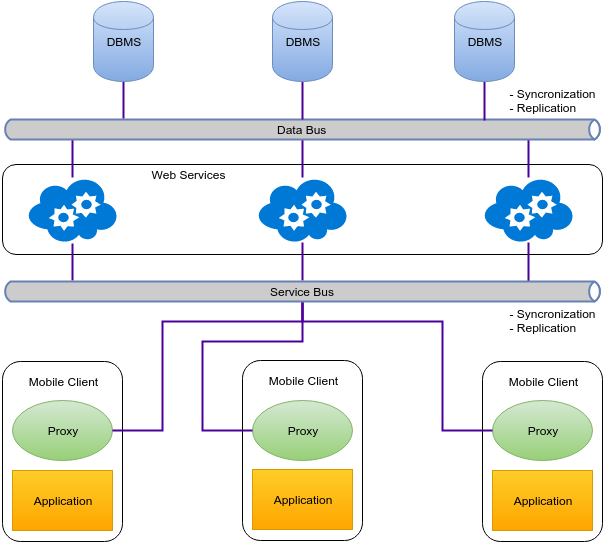
\includegraphics[width=8.5cm]{../../Resources/Images/proxy-overview}
    \caption{Proxy Overview}
    \label{fig:proxy-overview}
\end{figure}

This paper will examine how to design a proxy that can be used in a condition connected or disconnected, which is divided into five sections. Section 1 is the background of this research. While the second section will discuss the literature review and research related to the design of the proxy. Section 3 will discuss the proposed design, followed by a discussion in section 4. Finally section 5 concludes the paper with a summary and a discussion of future work.




\section{Theoretical Background}
In general, the proxy can be said as a placeholder for other entities \cite{gamma_design_1995}. Due to its capability to intercept communication source and target, it allows deferring the initialization of the target, redirecting the communication target to one or more entities, performing additional capabilities before/after communicating with the target, etc. \cite{gani_improving_2009}.

Implementation of the proxy have been conducted with various purposes, e.g., for memory efficiency \cite{gamma_design_1995}, remote communication \cite{wilson_get_2000}, and concurrent data evaluation/processing (e.g. for future object) \cite{pratikakis_transparent_2004}. Proxies have also been used in component-based middleware such as EJB \cite{_fusion_????}, to provide various enterprise-level capabilities. Furthermore, proxies have also been widely adopted in contemporary work on application adaptation \cite{holder_system_1999} \cite{philippsen_javaparty_1997} \cite{rubinsztejn_framework_2005} \cite{ryan_application_2004} \cite{tatsubori_bytecode_2001} \cite{tilevich_j-orchestra:_2002}, since they allow certain components of an application to dynamically reconfigure themselves (e.g. changing its behavior) transparently, i.e. without the awareness of the rest of the components in the application. While on the mobile device, the proxy is used to bridge the wired-wireless gap, and make all mobility, connectivity and context-dependent issues transparent to the application developer \cite{rubinsztejn_framework_2005}.

To support the mobility of a mobile device, the proxy must also be portable and dynamic. Rubinsztejn et al make the architectural design of the proxy in the form of middleware, which consists of both server and client API \cite{rubinsztejn_framework_2005} called MoCA. MoCA architecture consists of a monitor and several services. Monitor is a daemon or service that runs on each mobile client to collect and submit data to the services that run on the server side.

Another approach in the design of proxy proposed by Cobarzan et al. To support the dynamism of proxy, they composed proxy that consists of two components, the daemon and the dispatchers \cite{cobarzan_dynamic_2005}. Dispatcher is a component that acts as proxy. While Dispatcher is used to handle incoming client request, then forward them to the server or to other dispatchers, process it itself, or reject it. Meanwhile, the daemon is a component that runs automatically in the background and is used to monitor the code that contains the command to enable dispatchers. So that the proxy is not automatically activated by the daemon is active before, contrasts with the MoCA which automatically activates the proxy.

Proxy has several functions, such as content adaptation, protocol translation, user authentication, handover management, and cache management \cite{rubinsztejn_framework_2005}. Cache has an important role in reducing latency and network traffic between server and client \cite{rizzo_replacement_2000}. Caching can be implemented in several locations: at the client \cite{bestavros_application-level_1995} \cite{cao_cost-aware_1997}, server \cite{arlitt_trace-driven_1997} \cite{bestavros_application-level_1995}, and within the network \cite{abrams_caching_1995} \cite{cao_cost-aware_1997} \cite{busari_sensitivity_2001} through a proxy server.

Caching is generally implemented on a web the document to store frequently accessed parts of the document \cite{mahanti_temporal_2000} \cite{shim_proxy_1999-1} \cite{busari_sensitivity_2001}, either dynamic or static web contents, although not uncommon also implemented at the application level \cite{holder_system_1999} \cite{philippsen_javaparty_1997} \cite{rubinsztejn_framework_2005}. Since the cache is a temporary object \cite{davison_survey_1999} that represents the data on the server, it needs a method to ensure the consistency of data stored in the cache and which are contained in the server.

Caching method in a distributed system, including on a mobile devices, have a different design with a centralized system. Takdir et al proposed a method of proxy, by caching both data and workflow that will be used by the composite application on the local storage \cite{takdir_multi-layer_2014}. This method provides a transparent resources (i.e. the data and web service logics) access using combination of synchronization, replication, and routing mechanism.

Meanwhile, Terry et al using XML web services caching method \cite{terry_caching_2003} that mimics the behavior of Web services to a limited extent. This XML cache is transparent either on the client side and the server component on a Web services. This method is able to handle disconnections for each Web services. However, this method is lack of consistency, so that an operation performed by the local user could change some of the results of the earlier requests that are stored in the cache.

In a workflow-based application, such as the application of data collection, in which workflows are defined, managed, and executed in accordance with the sequence of logic \cite{wieland_towards_2009}, one of the standard that is now being widely used is the Business Process Execution Language (BPEL) \cite{pautasso_restful_2009} \cite{weerawarana_web_2005}, BPEL is built on the Web Service (WS) standards and Provides a recursive aggregation models for Web services \cite{pasley_how_2005} and used as glue between interacting services \cite{weerawarana_web_2005}. BPEL drives communication of web services in order to deliver business services that Contain several interconnected processes. Web services address interoperability issues in service level, whereas BPEL orchestrate web services in process level. BPEL is ideally suited to the service-oriented architecture, a set of guidelines for integrating disparate systems by presenting each system as a service that implements a specific business function [29].

\begin{figure}
    \centering
    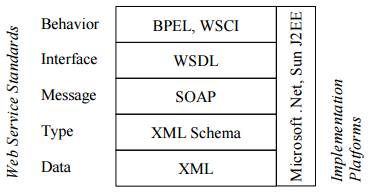
\includegraphics[width=8cm]{../../Resources/Images/ws-standards-stack}
    \caption{Web Service Standards Stack}
    \label{fig:ws-standards-stack}
\end{figure}




\section{Mobile Proxy Design}


\subsection{Design Overview}
Proposed proxy mobile design consists of three components, data, services, and applications, which are connected via two buses, the data bus and bus service. Illustration of design can be seen in \figurename{\ref{fig:proxy-overview}}.

Data bus Provides transparent access to the data source for web services. The data bus consists of two layers, ie cluster database layer and proxy layer. The cluster database layer consists of several database nodes that are equipped with a control cluster to ensure data synchronization. Meanwhile, the proxy layer consists of a proxy server that acts as a load balancer for database nodes. Load balancer is equipped with a healthy check to check the availability of each database node.

Similar with the data bus, the service bus handle web service invocation by the application. Web services that are representation of the rules, are packed as a bundle. Then the bundles are replicated, by composite application, from central repository to local repository. The bundles that are available in local repository will be installed and started dynamically by composite application. Moreover, installed bundles can also be stopped, removed, and updated easily.

\begin{figure}
    \centering
    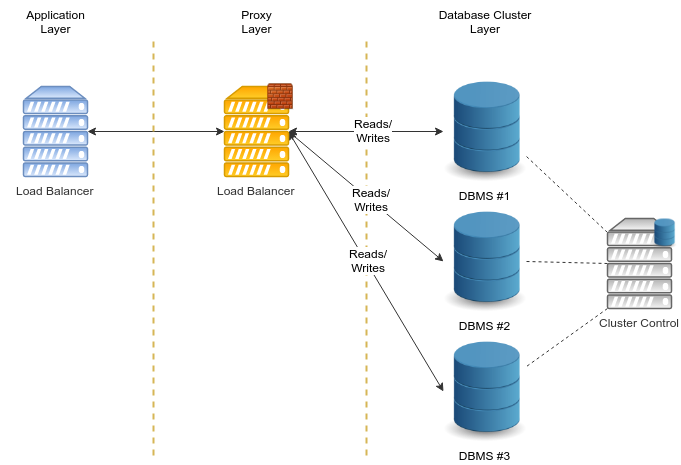
\includegraphics[width=8cm]{../../Resources/Images/proxy-design-data-layers}
    \caption{Data Bus Layers}
    \label{fig:proxy-design-data-layers}
\end{figure}




\subsection{Replication}
Data and web services bundles are replicated from central storage to local storage as cache objects. Firstly, composite application replicate web services bundles from central repository to local repository. Each web services bundle then will replicate data that it is depend on, from central database into local storage. \figurename{\ref{fig:replication-flowchart}} shows web services and data replication strategy.

\begin{figure}
	\centering
	\subfloat[Web Services Replication Strategy]{
		\centering
		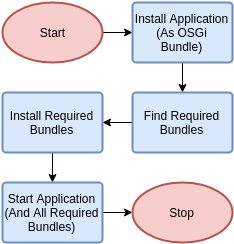
\includegraphics[width=3.5cm]{../../Resources/Images/bundle-replication-flowchart}
		\label{fig:bundle-replication-flowchart}
	}
	\hfil\hfil
	\subfloat[Data Replication Strategy]{
		\centering
		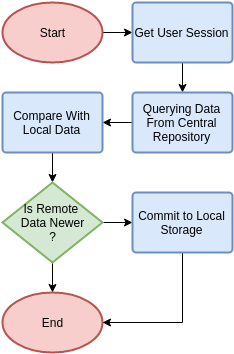
\includegraphics[width=3.5cm]{../../Resources/Images/data-replication-flowchart}
		\label{fig:data-replication-flowchart}}
	\caption{Replication Strategies}
	\label{fig:replication-flowchart}
\end{figure}




\subsection{Synchronization}
Synchronization ensure the data and web service bundles are consistent between local and central repository. Web service bundle must implement versioning, so central server and proxy server must install bundles with same version to ensure the same logic is used. Composite application will periodically execute version check of the bundles, and replicate it when new versions are available in central repository.

Data synchronization is very depend on bundle, since each bundle require different data. Data will be synchronized in two way, from central database to local cache storage (e.g. master data) and from local cache storage to central storage (e.g. transaction data). \figurename{\ref{fig:data-sync-flowchart}} shows data syncronization strategy.

\begin{figure}
    \centering
    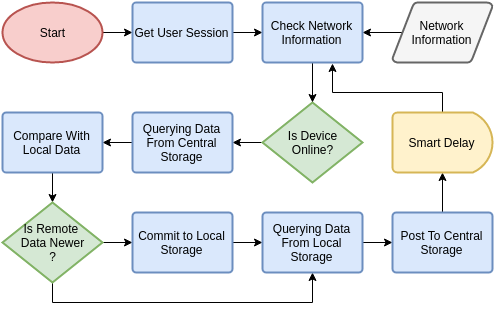
\includegraphics[width=8cm]{../../Resources/Images/data-sync-flowchart}
    \caption{Data Syncronization Strategy}
    \label{fig:data-sync-flowchart}
\end{figure}




\subsection{Routing}
Routing plays important role in distributed system. It manages the network traffic and point requests to appropriate destination \cite{takdir_multi-layer_2014}. Local web services are act as proxy server that intermediate composite application, that act as client, and central server. Proxy server will decide whether to forward request to central server or reply it on behalf of central server. \figurename{\ref{fig:routing-flowchart}} shows routing strategy.

\begin{figure}
    \centering
    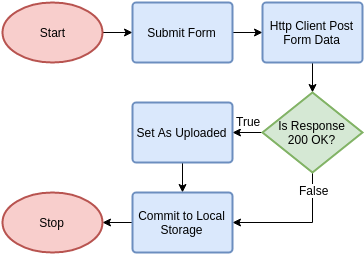
\includegraphics[width=6cm]{../../Resources/Images/routing-flowchart}
    \caption{Routing Strategy}
    \label{fig:routing-flowchart}
\end{figure}



\section{Implementation}


\subsection{OSGi Framework}
There are several implementations of OSGi, or commonly referred to OSGi Framework, ie: Apache Felix, Concierge, Equinox Eclipse, JBoss, Hitachi, Knopflerfish, and ProSyst. This study uses the Knopflerfish OSGi Framework, because Knopflerfish OSGi Framework has implemented the latest OSGi specification, the OSGi R6. In addition, the Knopflerfish OSGi Framework is also proven to be implemented in Android application.




\subsection{Android Application} \label{ssec:android-application}
By default, Knopflerfish provides an implementation of the OSGi Framework that can be run on any operating system that supports Java SE. However, because the Android OS uses a different JVM implementations, the Dalvik VM, so it needs to be made Knopflerfish OSGi Framework implementations that can run on the Android OS.

Android application that is made must support the principle of OSGi, which is modular. The case studies used in this study is a case study for field data collection, so that the user interface is a questionnaire form. To accelerate the creation and simplify the loading of the page, so it is used Cordova. Cordova is a webview-based, so the control used is an HTML form element. \figurename{\ref{fig:android-app}} shows screenshots of Android application.

\begin{figure}
	\centering
	\subfloat[Home Page]{
		\centering
		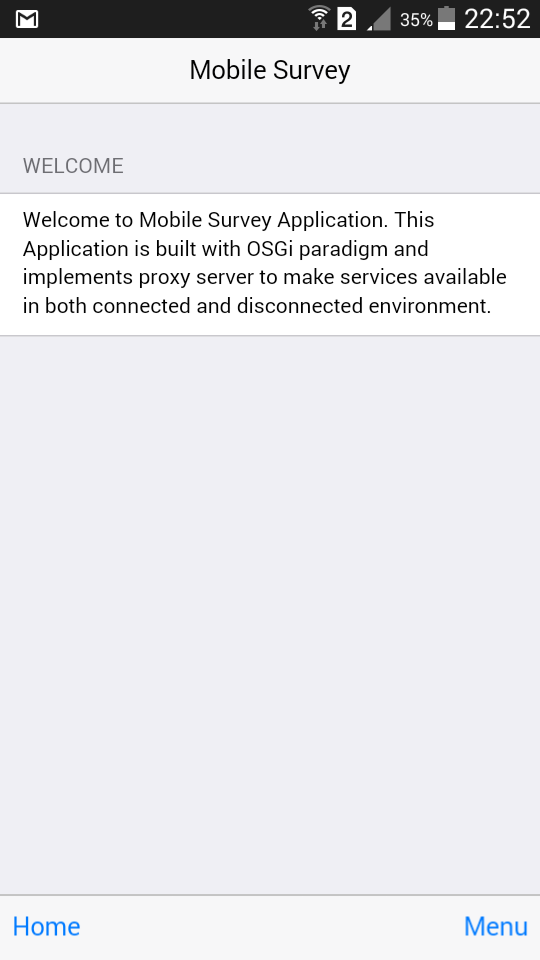
\includegraphics[width=2.5cm]{../../Resources/Images/android-app-1}
		\label{fig:android-app-1}
	}
	\hfil
	\subfloat[Autostart OSGi Framework]{
		\centering
		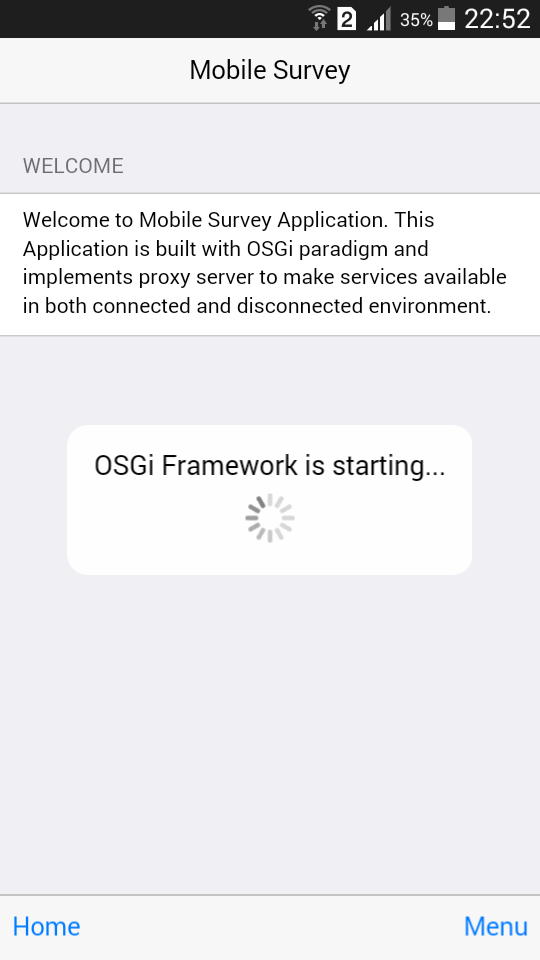
\includegraphics[width=2.5cm]{../../Resources/Images/android-app-2}
		\label{fig:android-app-2}}
	\hfil
	\subfloat[Bundle Page]{
		\centering
		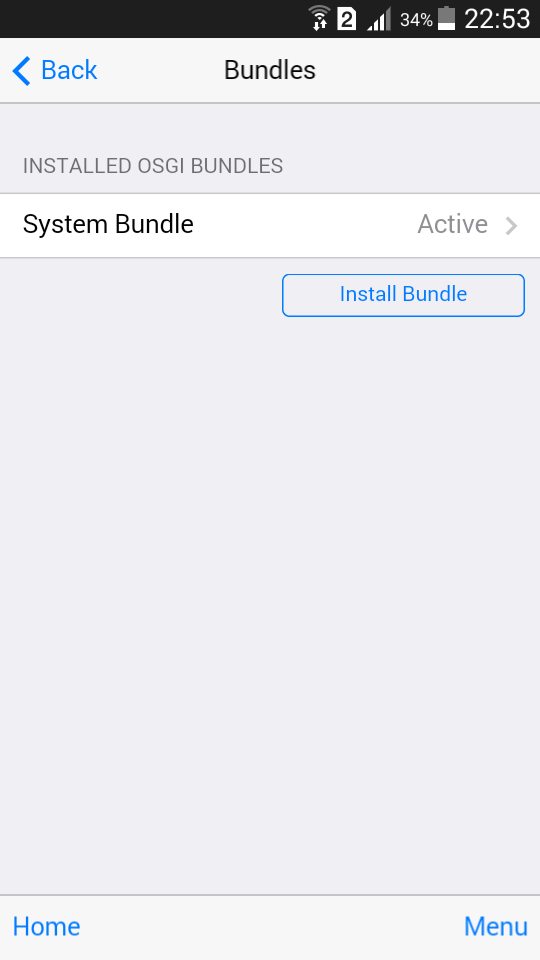
\includegraphics[width=2.5cm]{../../Resources/Images/android-app-3}
		\label{fig:android-app-3}}
	\caption{Android Application}
	\label{fig:android-app}
\end{figure}




\subsection{OSGi Bundles}

\subsubsection{Proxy Server}
Proxy server is an OSGi bundle that implements an embedded web server. Web server used in this study is Jetty 9 which is the highest major version available today. In the Proxy Server Bundle registered a service (API) ContextHandlerService, which is used to register the ServletContext initiated on Application Bundle.

\subsubsection{Composite Application}
Composite Application is an OSGi bundle that implements web services and clients in a same bundle. Web services are implemented in the form of Servlets collected in a single context. While the client is implemented in the form of a web-based application, written in HTML, Javascript, and CSS. In addition, the Composite Application also provides an API that can be imported dynamically by another bundle, ie: AccountHandlerService, DaoHandlerService, and PropertyHandlerService.

\subsubsection{Synchronizer}
Synchronizer is an OSGi bundle that is used to synchronize data in two directions: Remote to Local and Local to Remote. Synchronizer bundle requires some service provided by Composite Application, ie: AccountHandlerService to access the session to be synchronized and DaoHandlerService to access local storage.

\figurename{\ref{fig:android-bundle}} shows screenshots of OSGi bundles installed and started in Android environment.

\begin{figure}
	\centering
	\subfloat[Install bundle]{
		\centering
		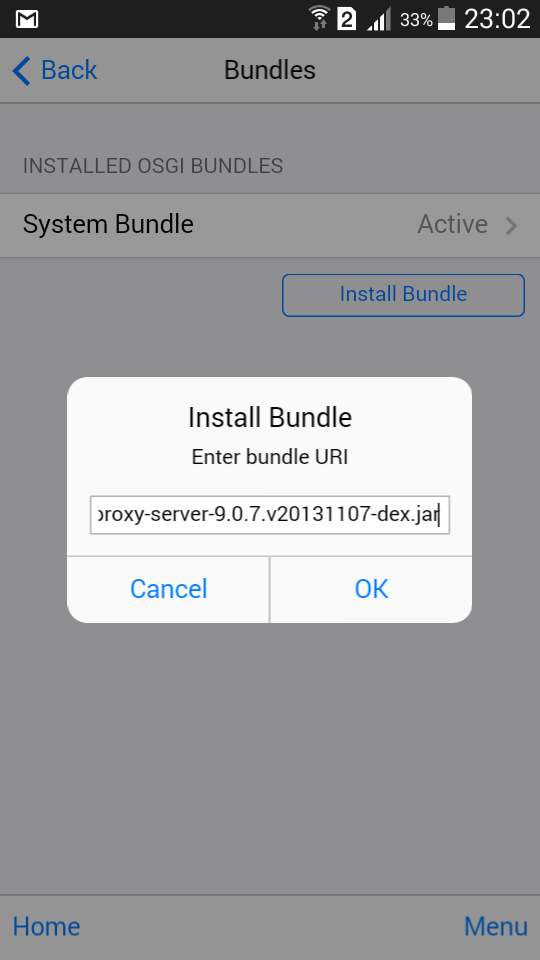
\includegraphics[width=2.5cm]{../../Resources/Images/android-bundle-1}
		\label{fig:android-bundle-1}}
	\hfil
	\subfloat[Bundle is installing]{
		\centering
		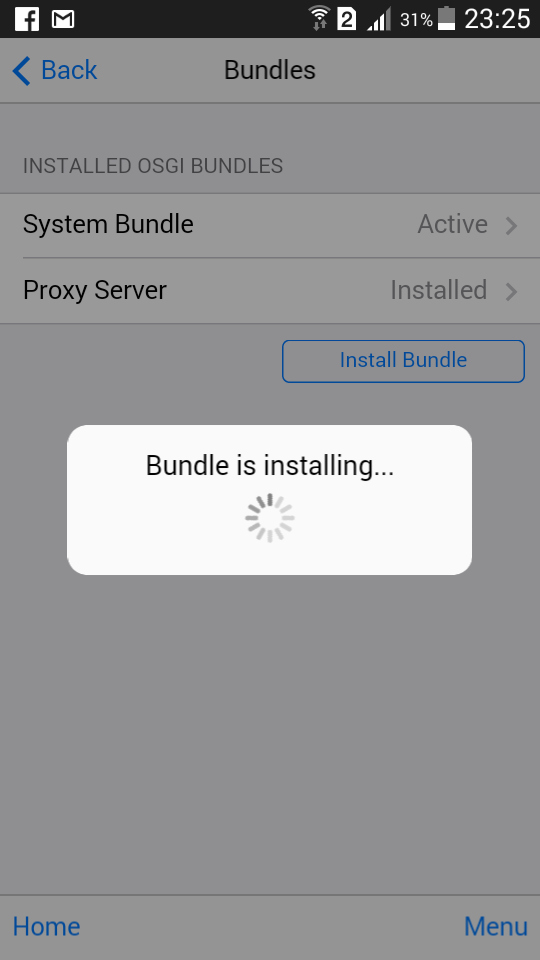
\includegraphics[width=2.5cm]{../../Resources/Images/android-bundle-2}
		\label{fig:android-bundle-2}}
	\hfil
	\subfloat[Bundles are installed]{
		\centering
		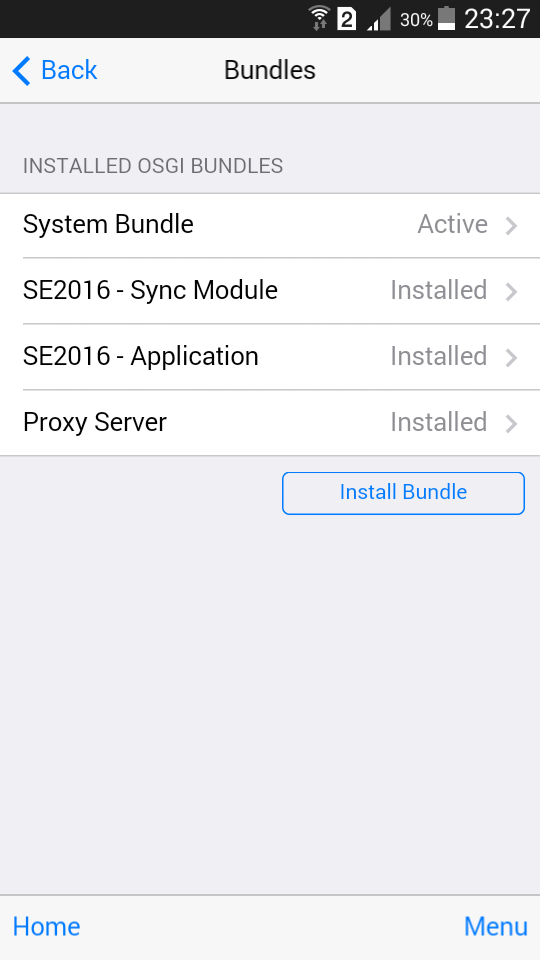
\includegraphics[width=2.5cm]{../../Resources/Images/android-bundle-3}
		\label{fig:android-bundle-3}}
	\vfil
	\subfloat[Bundle is starting]{
		\centering
		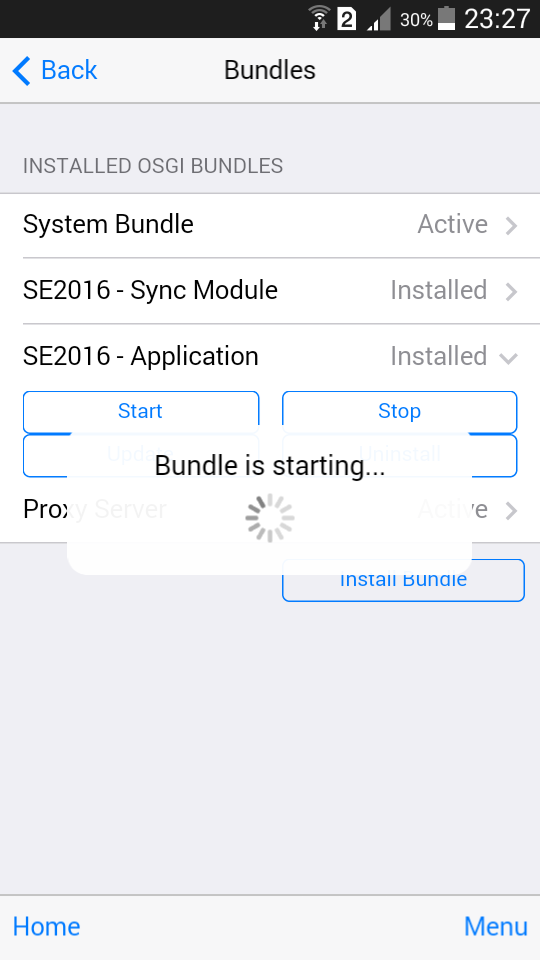
\includegraphics[width=2.5cm]{../../Resources/Images/android-bundle-4}
		\label{fig:android-bundle-4}}
	\hfil
	\subfloat[Bundles are active]{
		\centering
		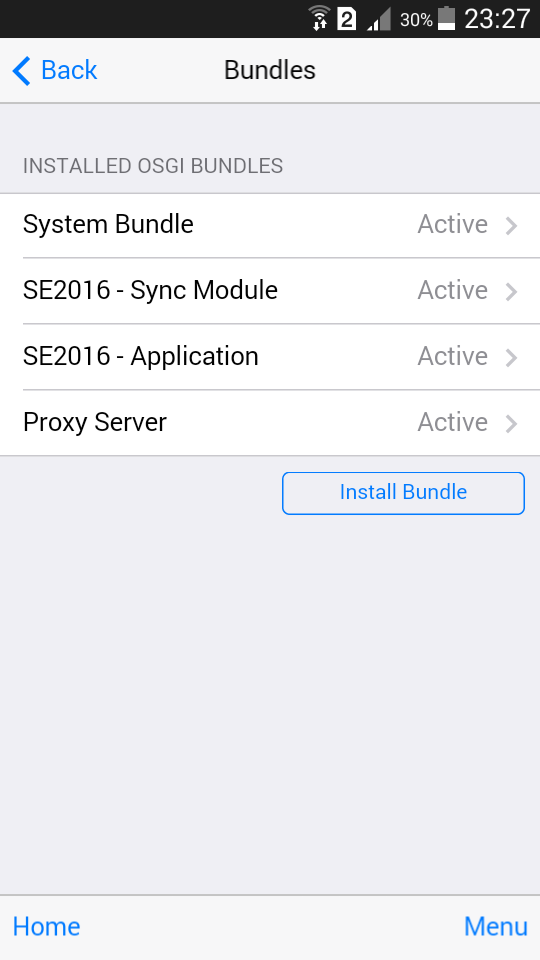
\includegraphics[width=2.5cm]{../../Resources/Images/android-bundle-5}
		\label{fig:android-bundle-5}}
	\hfil
	\subfloat[Composite application is loaded]{
		\centering
		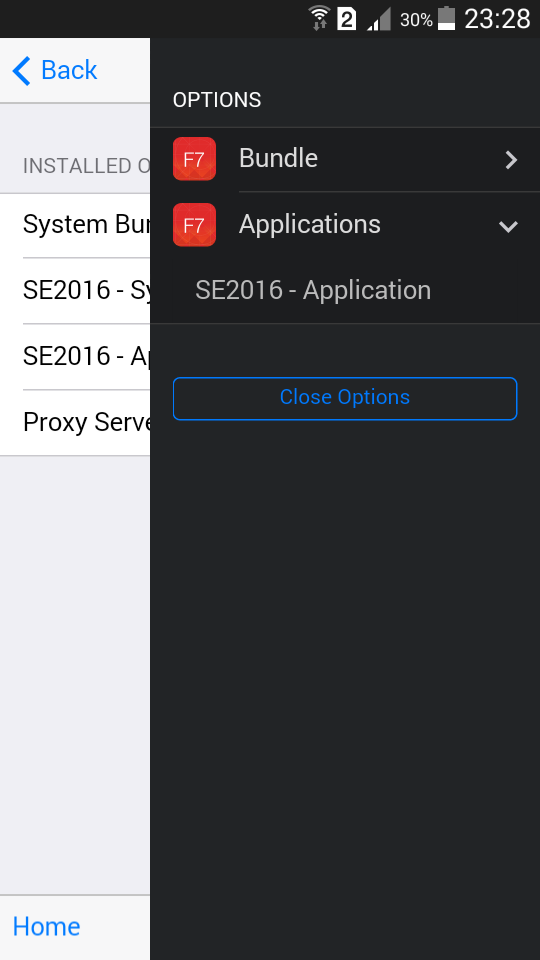
\includegraphics[width=2.5cm]{../../Resources/Images/android-bundle-6}
		\label{fig:android-bundle-6}}
	\caption{Android Bundles}
	\label{fig:android-bundle}
\end{figure}




\subsection{Remote Server}
As described in \ref{ssec:android-application}, Knopflerfish by default already provides an implementation of the OSGi Framework that can be run on any operating system that supports Java SE. Remote server running Knopflerfish using minimal bundle, and installed the same module with the composite application. Listing.\ref{lst:start-framework-remote} and Listing.\ref{lst:start-bundle-remote} shows screenshots of OSGi bundles are active in remote server.

\begin{listing}
    \caption{Knopflerfish with minimal bundles}
    \begin{minted}[showspaces=false,breaklines=true]{java}
java -jar framework.jar -xargs minimal.xargs
Knopflerfish OSGi framework launcher, version <unknown>
Copyright 2003-2015 Knopflerfish. All Rights Reserved.
See http://www.knopflerfish.org for more information.

Created Framework: org.knopflerfish.framework, version=7.2.0.
> Framework launched
	\end{minted}
    \label{lst:start-framework-remote}
\end{listing}

\begin{listing}
    \caption{Install and start required bundles}
    \begin{minted}[showspaces=false,breaklines=true]{java}
> install http://knopflerfish.soedomoto.tk/ jars/pgfw7/proxy-server-9.0.7.v20131107- dex.jar
Installed: Proxy Server (#10)
> start 10
2016-09-05 21:57:02.294:INFO:oejs.Server: BundleStart #10: jetty-9.0.z-SNAPSHOT
2016-09-05 21:57:02.455:INFO:oejs. ServerConnector: BundleStart #10: Started ServerConnector@698b6705 {HTTP/1.1}{0.0.0.0:5555}
Started: Proxy Server (#10)
> install http://knopflerfish.soedomoto.tk/ jars/pgfw7/se2016-bundle-0.1-SNAPSHOT- dex.jar
Installed: SE2016 - Application (#11)
> start 11
...
2016-09-05 21:57:33.147:INFO:oejsh. ContextHandler:BundleStart #11: Started o.e.j.s.ServletContextHandler@390161c7 {/se2016,null,AVAILABLE}
Started: SE2016 - Application (#11)
> install http://knopflerfish.soedomoto.tk/ jars/pgfw7/se2016-sync-bundle-0.1- SNAPSHOT-dex.jar
Installed: SE2016 - Sync Module (#12)
> start 12
Started: SE2016 - Sync Module (#12)
...
	\end{minted}
    \label{lst:start-bundle-remote}
\end{listing}




% An example of a floating figure using the graphicx package.
% Note that \label must occur AFTER (or within) \caption.
% For figures, \caption should occur after the \includegraphics.
% Note that IEEEtran v1.7 and later has special internal code that
% is designed to preserve the operation of \label within \caption
% even when the captionsoff option is in effect. However, because
% of issues like this, it may be the safest practice to put all your
% \label just after \caption rather than within \caption{}.
%
% Reminder: the "draftcls" or "draftclsnofoot", not "draft", class
% option should be used if it is desired that the figures are to be
% displayed while in draft mode.
%
%\begin{figure}[!t]
%\centering
%\includegraphics[width=2.5in]{myfigure}
% where an .eps filename suffix will be assumed under latex, 
% and a .pdf suffix will be assumed for pdflatex; or what has been declared
% via \DeclareGraphicsExtensions.
%\caption{Simulation results for the network.}
%\label{fig_sim}
%\end{figure}

% Note that the IEEE typically puts floats only at the top, even when this
% results in a large percentage of a column being occupied by floats.


% An example of a double column floating figure using two subfigures.
% (The subfig.sty package must be loaded for this to work.)
% The subfigure \label commands are set within each subfloat command,
% and the \label for the overall figure must come after \caption.
% \hfil is used as a separator to get equal spacing.
% Watch out that the combined width of all the subfigures on a 
% line do not exceed the text width or a line break will occur.
%
%\begin{figure*}[!t]
%\centering
%\subfloat[Case I]{\includegraphics[width=2.5in]{box}%
%\label{fig_first_case}}
%\hfil
%\subfloat[Case II]{\includegraphics[width=2.5in]{box}%
%\label{fig_second_case}}
%\caption{Simulation results for the network.}
%\label{fig_sim}
%\end{figure*}
%
% Note that often IEEE papers with subfigures do not employ subfigure
% captions (using the optional argument to \subfloat[]), but instead will
% reference/describe all of them (a), (b), etc., within the main caption.
% Be aware that for subfig.sty to generate the (a), (b), etc., subfigure
% labels, the optional argument to \subfloat must be present. If a
% subcaption is not desired, just leave its contents blank,
% e.g., \subfloat[].


% An example of a floating table. Note that, for IEEE style tables, the
% \caption command should come BEFORE the table and, given that table
% captions serve much like titles, are usually capitalized except for words
% such as a, an, and, as, at, but, by, for, in, nor, of, on, or, the, to
% and up, which are usually not capitalized unless they are the first or
% last word of the caption. Table text will default to \footnotesize as
% the IEEE normally uses this smaller font for tables.
% The \label must come after \caption as always.
%
%\begin{table}[!t]
%% increase table row spacing, adjust to taste
%\renewcommand{\arraystretch}{1.3}
% if using array.sty, it might be a good idea to tweak the value of
% \extrarowheight as needed to properly center the text within the cells
%\caption{An Example of a Table}
%\label{table_example}
%\centering
%% Some packages, such as MDW tools, offer better commands for making tables
%% than the plain LaTeX2e tabular which is used here.
%\begin{tabular}{|c||c|}
%\hline
%One & Two\\
%\hline
%Three & Four\\
%\hline
%\end{tabular}
%\end{table}


% Note that the IEEE does not put floats in the very first column
% - or typically anywhere on the first page for that matter. Also,
% in-text middle ("here") positioning is typically not used, but it
% is allowed and encouraged for Computer Society conferences (but
% not Computer Society journals). Most IEEE journals/conferences use
% top floats exclusively. 
% Note that, LaTeX2e, unlike IEEE journals/conferences, places
% footnotes above bottom floats. This can be corrected via the
% \fnbelowfloat command of the stfloats package.




\section{Testing}
\subsection{Response Time}
Pengujian terhadap response time digunakan untuk mengukur latency antara client dan server. Pengujian ini menggunakan dua skenario, yaitu skenario tanpa proxy dan dengan proxy. Dari empat kali pengujian dengan jumlah transaksi yang bervariasi, seperti yang ditunjukkan dalam Table \ref{tbl:response_time}, menunjukkan dengan menggunakan proxy dapat mengurangi response time sebanyak 20 kali lipat dibandingkan dengan tanpa menggunakan proxy.


\begin{table}
\renewcommand{\arraystretch}{1.3}
\caption{Response Time Test (ms)}
\label{tbl:response_time}
\centering
\begin{tabular}{|c||c|c|c|c|c|c|}
\hline
Transactions & \multicolumn{3}{c|}{Without Proxy} & \multicolumn{3}{c|}{With Proxy}\\
\hline
& Total & $\mu$ & $\sigma$ & Total & $\mu$ & $\sigma$\\
\hline
11 & 4226 & 384.18 & 77.10 & 862 & 78.36 & 224.09\\
\hline
110 & 41999 & 381.81 & 51.54 & 1376 & 12.51 & 9.41\\
\hline
1100 & 405892 & 368.99 & 59.95 & 15891 & 14.45 & 13.47\\
\hline
5500 & 2226949 & 404.90 & 206.73 & 64600 & 11.74 & 9.92\\
\hline
\end{tabular}
\end{table}




\section{Conclusion and Future Work}
We propose a mobile proxy design that is dynamic, which can be distributed separately with composite applications and its synchronization. Distribution of proxy server, composite applications, and synchronization is done in the form of OSGi bundle. By adopting the principles of OSGi, synchronization workflows in the form of web services proved to be more effective, because each bundle can be updated independently, either manually or automatically.

By adopting the synchronization in a separate module also proven to be able to synchronize with better and more controlled because it can be start-stop and in every moment. Synchronization modules can also be updated, either manually or automatically, without affecting the other modules.

Our proposed design also makes it possible to install more than one composite applications and synchronization in an application with just a single proxy server.




% conference papers do not normally have an appendix


% use section* for acknowledgment
% \section*{Acknowledgment}
% The authors would like to thank...





% trigger a \newpage just before the given reference
% number - used to balance the columns on the last page
% adjust value as needed - may need to be readjusted if
% the document is modified later
%\IEEEtriggeratref{8}
% The "triggered" command can be changed if desired:
%\IEEEtriggercmd{\enlargethispage{-5in}}

% references section

% can use a bibliography generated by BibTeX as a .bbl file
% BibTeX documentation can be easily obtained at:
% http://mirror.ctan.org/biblio/bibtex/contrib/doc/
% The IEEEtran BibTeX style support page is at:
% http://www.michaelshell.org/tex/ieeetran/bibtex/
% bibliographystyle{IEEEtran}
% argument is your BibTeX string definitions and bibliography database(s)
% bibliography{IEEEabrv,Paper.bib}
%
% <OR> manually copy in the resultant .bbl file
% set second argument of \begin to the number of references
% (used to reserve space for the reference number labels box)
% \begin{thebibliography}{1}

% \bibitem{IEEEhowto:kopka}
% H.~Kopka and P.~W. Daly, \emph{A Guide to \LaTeX}, 3rd~ed.\hskip 1em plus
%   0.5em minus 0.4em\relax Harlow, England: Addison-Wesley, 1999.

% \end{thebibliography}

\bibliographystyle{IEEEtran}
\bibliography{IEEEabrv,../../Resources/Bibliography/Paper.bib}


% that's all folks
\end{document}


